\clearpage % Rozdziały zaczynamy od nowej strony.
\section{Realizacja Pracowni}

\subsection{Harmonogram prac}

Na początku semestru został sporządzony harmonogram prac, który został przedstawiony w tabeli \ref{table:harmonogram}.

\begin{longtable}{| m{0.67\linewidth} | r |}
    \caption{Harmonogram prac.}
    \label{table:harmonogram} \\

    \hline
    % Nagłówek tabeli wyrównujemy do środka
    \multicolumn{1}{|c|}{Kamień milowy} & \multicolumn{1}{c|}{Przewidywana data ukończenia} \\ \hline\hline \endfirsthead \endfoot
    \hline \endlastfoot

    Zamodelowanie zdarzeń biznesowych przy pomocy techniki Event Storming & 27.03.2023 \\ \hline
    Wstępny wybór technologii & 17.04.2023 \\ \hline
    Przygotowanie środowiska programistycznego & 24.04.2023 \\ \hline
    Weryfikacja wykorzystania wybranych technologii & 8.05.2023 \\ \hline
    Ustalenie wymagań funkcjonalnych i niefunkcjonalnych & 22.05.2023 \\ \hline
    Wykonanie makiet interfejsu użytkownika & 5.06.2023 \\ \hline
    Ustalenie formatów i technik wymiany danych & 12.06.2023 \\ \hline
    Przygotowanie mechanizmów uwierzytelniania i autoryzacji użytkowników & 19.06.2023 \\ \hline
    Zaprojektowanie architektury i infrastruktury aplikacji & 26.06.2023 \\ \hline
    Główna implementacja & 2.10.2023 \\ \hline
    Wdrożenie produkcyjne aplikacji & 9.10.2023 \\ \hline
    Przygotowanie i wykonanie automatycznych testów akceptacyjnych & 23.10.2023 \\ \hline
    Przygotowanie i wykonanie automatycznych testów wydajnościowych & 6.11.2023\\ \hline
    Przygotowanie raportu z wydajności i skalowalności systemu & 13.11.2023 \\ \hline
    Przygotowanie wstępnego tekstu pracy inżynierskiej & 18.12.2023 \\ \hline
    Przygotowanie finalnego tekstu pracy inżynierskiej & 8.01.2024 \\ \hline
    Złożenie pracy inżynierskiej & 15.01.2024 \\ \hline
\end{longtable}

Zakres Pracowni Dyplomowej 1 zakończył się wraz z ukończeniem kamienia milowego \textit{Wykonanie makiet interfejsu użytkownika}.

% Podrozdział pierwszego poziomu
\subsection{Zamodelowanie zdarzeń biznesowych}

\subsubsection{Wstęp}

W celu zrozumienia procesów oraz zidentyfikowania potencjalnych mikroserwisów w tworzonej aplikacji, przeprowadzono sesję Event Stormingu. Metoda ta umożliwia wizualizację i modelowanie procesów biznesowych w ramach systemu, co jest kluczowe przy tworzeniu złożonych systemów informatycznych. W niniejszym rozdziale przedstawione zostaną wyniki sesji Event Stormingu, która została przeprowadzona z wykorzystaniem narzędzia Miro.

\subsubsection{Narzędzie Miro}

Miro to interaktywna platforma do współpracy, umożliwiająca tworzenie tablic z notatkami, rysunkami i diagramami. Wybór tego narzędzia był podyktowany jego prostotą użytkowania oraz możliwościami wizualizacji modelu związanego z Event Stormingiem.

\subsubsection{Identyfikacja kontekstów granicznych (Bounded Context)}

W wyniku sesji Event Stormingu zidentyfikowano pięć kontekstów granicznych (Bounded Context), które będą kluczowe dla tworzonej aplikacji. Są to:

\begin{itemize}
    \item Restaurant - obejmuje zarządzanie restauracjami, menu i dostępnością produktów
    \item Order - odpowiada za proces zamówienia, takie jak składanie, modyfikowanie i anulowanie zamówień
    \item Delivery - koncentruje się na logistyce dostaw, monitorowaniu statusu dostawy oraz komunikacji z dostawcą. Zarządza również bazą dostawców
    \item Payment - zarządza procesem płatności, obejmuje różne metody płatności oraz obsługę transakcji. Obsługuje wszelkie rozliczenia w ramach systemu
    \item User - dotyczy zarządzania kontami użytkowników, uwierzytelniania oraz zarządzania uprawnieniami
    \item Invoice - odpowiada za generowanie faktur
\end{itemize}

\subsubsection{Analiza procesów}


Każdy z wyżej wymienionych kontekstów granicznych został poddany analizie procesów, które występują w ramach danej domeny. W trakcie analizy zidentyfikowano następujące kluczowe zdarzenia:

\begin{itemize}
    \item Restaurant
    \begin{itemize}
        \item Dodanie nowej restauracji
        \item Aktualizacja informacji o restauracji
        \item Dodanie/aktualizacja menu
        \item Zmiana dostępności restauracji
        \item Przyjęcie lub odrzucenie zamówienia przez restaurację
        \item Aktualizacja statusu zamówienia (gotowe do odbioru)
    \end{itemize}
    
    \item Order
    \begin{itemize}
        \item Utworzenie nowego zamówienia
        \item Modyfikacja zamówienia
        \item Anulowanie zamówienia
        \item Finalizacja zamówienia
    \end{itemize}
    
    \item Delivery
    \begin{itemize}
        \item Dodanie nowego dostawcy
        \item Aktualizacja informacji o dostawcy
        \item Zmiana dostępności dostawy
        \item Przypisanie dostawcy do zamówienia
        \item Wytyczenie trasy dostawy
        \item Odbiór zamówienia przez dostawcę
        \item Dostarczenie zamówienia do klienta
    \end{itemize}
    
    \item Payment
    \begin{itemize}
        \item Przyjęcie płatności za zamówienie
        \item Obsługa nieudanej płatności
        \item Rozliczenie płatności z dostawcą
        \item Rozliczenie płatności z restauracją
        \item Obsługa zwrotu płatności w przypadku anulowania zamówienia
        \item Wypłata środków do restauracji
        \item Wypłata środków do dostawcy
    \end{itemize}
    
    \item User
    \begin{itemize}
        \item Rejestracja nowego użytkownika
        \item Logowanie użytkownika
        \item Aktualizacja danych użytkownika (metody płatności, adresy dostawy, preferencje)
        \item Usunięcie konta użytkownika
    \end{itemize}
    
    \item Invoice
    \begin{itemize}
        \item Generowanie faktury dla restauracji
        \item Generowanie faktury dla dostawcy
        \item Generowanie faktury dla zamawiającego
    \end{itemize}
\end{itemize}


\subsubsection{Reprezentacja graficzna}

Na rysunku \ref{fig:event-storming} przedstawiono wynik sesji Event Stormingu w postaci diagramu wygenerowanego przy pomocy narzędzia Miro.

\begin{figure}[!h]
    \centering 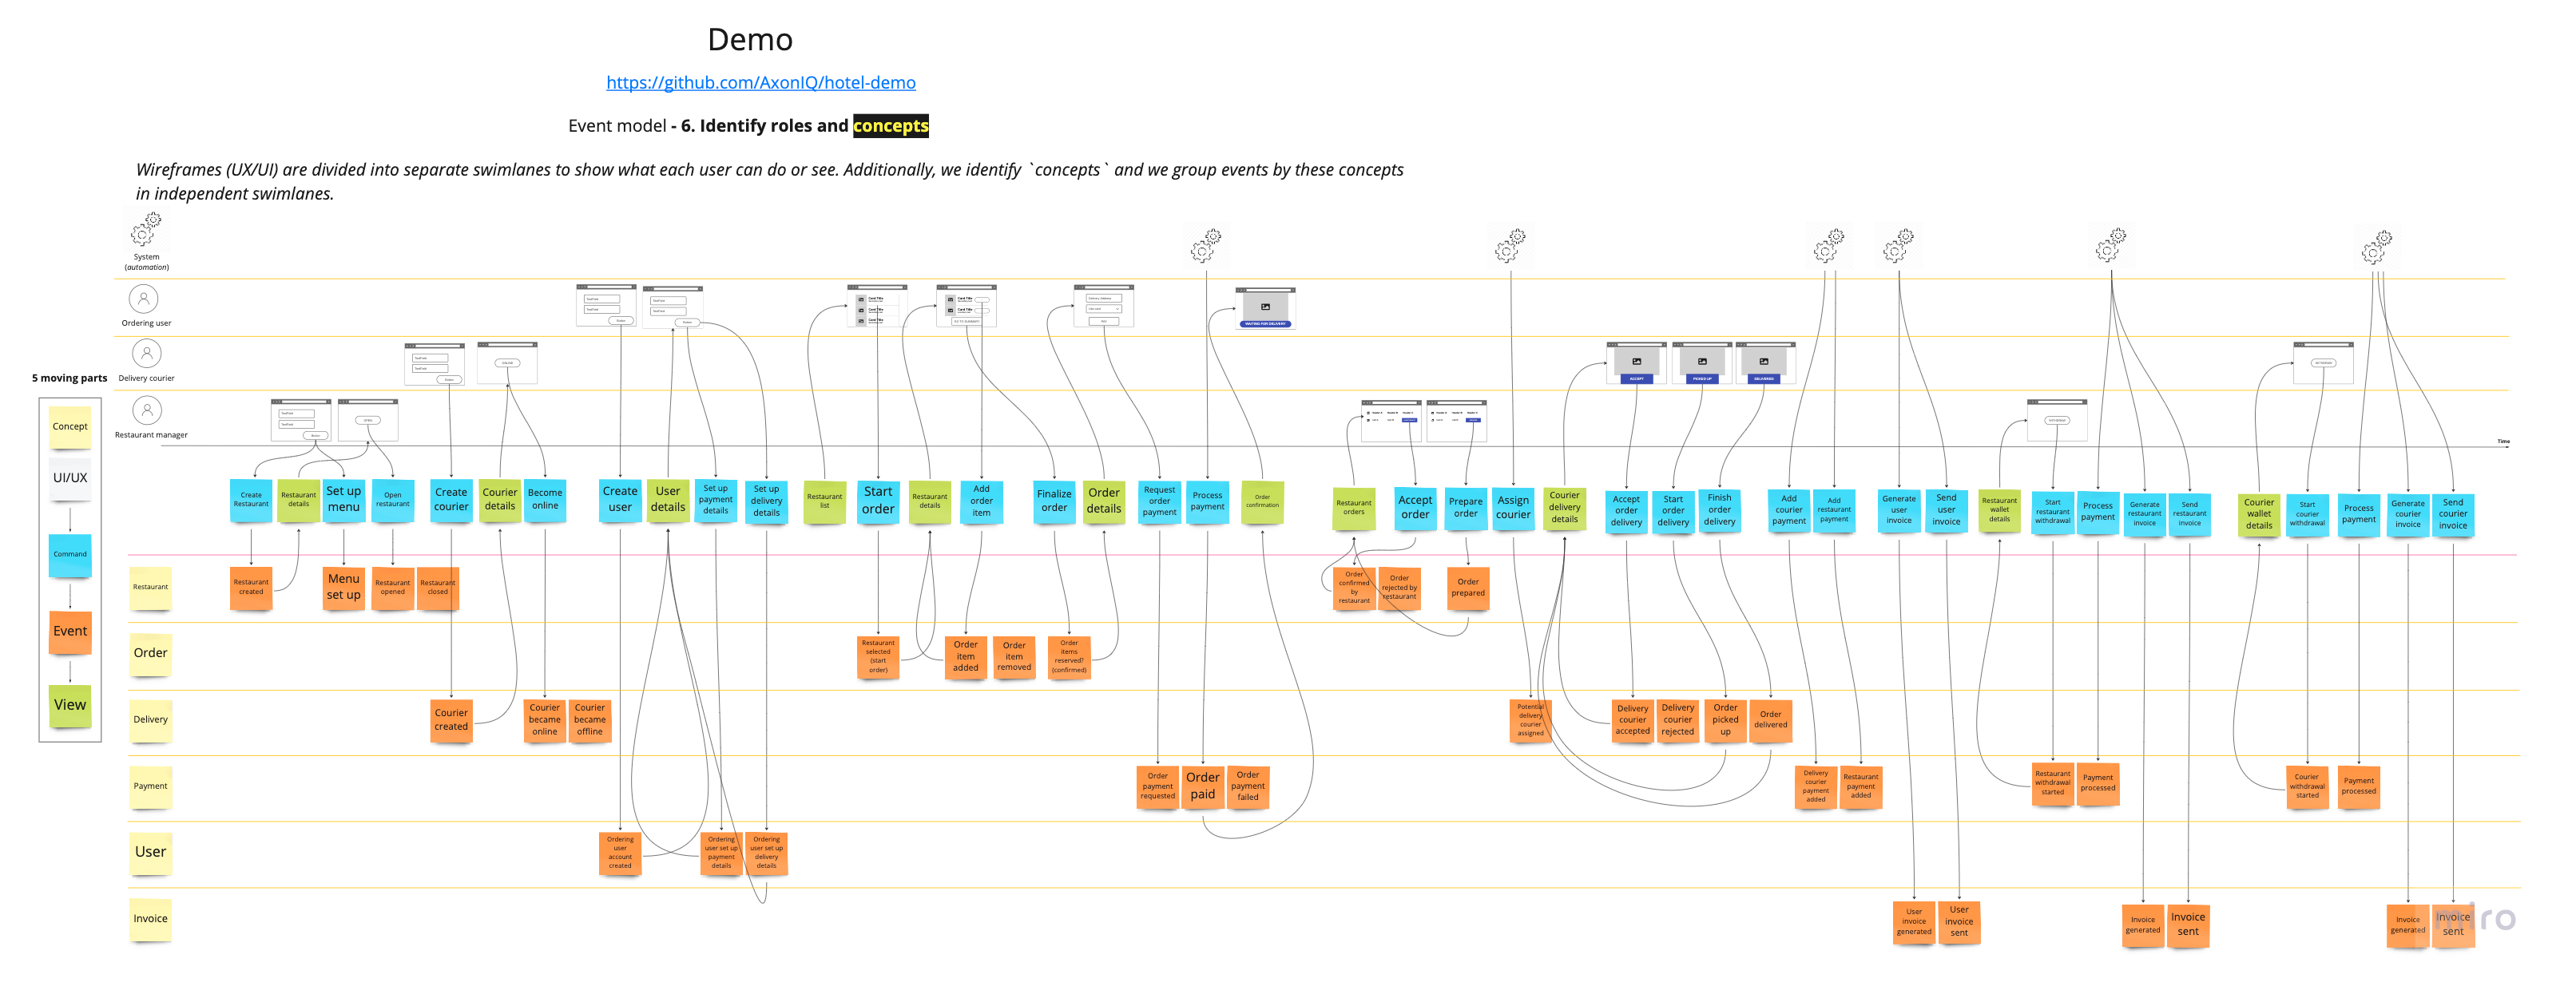
\includegraphics[width=1.0\linewidth]{event_storming.png}
    \caption{Reprezentacja graficzna efektów sesji Event Stormingu}
    \label{fig:event-storming}
\end{figure}



% Nagłówki kolejnych poziomów, dla zapełnienia spisu treści
\subsection{Wstępny wybór technologii}

Całość rozwiązania została wdrożona przy pomocy narzędzia Kubernetes. W celu zautomatyzowania procesu wdrażania wykorzystano platformę Ciągłej Integracji/Ciągłego Wdrażania GitHub Actions. W celu monitorowania oraz obserwalności aplikacji wykorzystano narzędzie Prometheus, Grafana oraz Loki.

\subsubsection{Część serwerowa}

Język programowania: Kotlin

Frameworki: Axon Framework + Spring Boot

Format komunikacji: JSON (REST)

Baza danych: MongoDB

\subsubsection{Część kliencka}

Język programowania: TypeScript

Framework: Remix + React

\subsection{Przygotowanie środowiska programistycznego}

W celu efektywnej pracy nad projektem przygotowano środowisko programistyczne używane do rozwoju i wdrożenia aplikacji. Środowisko programistyczne można podzielić na dwa rodzaje: lokalne i zdalne (wdrożeniowe).

\subsubsection{Środowisko lokalne}

Środowisko lokalne składa się z następujących elementów:

\begin{itemize}
    \item System operacyjny: MacOS
    \item Zintegrowane środowisko programistyczne (IDE): IntelliJ IDEA
    \item Środowisko uruchomieniowe: Docker + Docker Compose
\end{itemize}

IDE IntelliJ IDEA jest używane do pisania, testowania i debugowania kodu. Docker i Docker Compose służą do tworzenia i zarządzania skonteneryzowanymi środowiskami dla aplikacji.

\subsubsection{Środowisko wdrożeniowe}

Środowisko zdalne jest używane do wdrożenia aplikacji do produkcji. Środowisko zdalne składa się z następujących elementów:

\begin{itemize}
    \item System operacyjny: Ubuntu 22.04
    \item Specyfikacja maszyny: 4vCPU, 12GB RAM, 50GB SSD
    \item Lokalizacja: Sztokholm, Szwecja
    \item Klaster Kubernetes: MicroK8s
\end{itemize}

Środowisko zdalne jest hostowane na maszynie o wyższych specyfikacjach, aby zapewnić płynne działanie aplikacji w produkcji. Lokalizacja maszyny to Sztokholm, Szwecja, a działa ona na klastrze Kubernetes MicroK8s. Klastry Kubernetes są używane do zarządzania wdrożeniem aplikacji w sposób skalowalny i niezawodny.

\subsection{Weryfikacja wykorzystania wybranych technologii}

Weryfikacja została przeprowadzona na przykładzie serwisów "Restaurant" i "Order", które są odpowiedzialny za zarządzanie listą restauracji, ich menu oraz zamówieniami. W ramach projektu zaimplementowano zarówno część serwerową, jak i kliencką.

Wybór technologii okazał się trafiony, co umożliwiło implementację wszystkich funkcjonalności w sposób prosty i intuicyjny. Ponadto, wybrane technologie umożliwiły łatwe rozszerzanie aplikacji o nowe funkcje.

Zbudowany fragment systemu został wdrożony na środowisko produkcyjne.

\subsubsection{Część serwerowa}

W ramach części serwerowej zaimplementowano następujące funkcjonalności:

\begin{itemize}
    \item Dodawanie restauracji
    \item Usuwanie restauracji
    \item Aktualizowanie informacji o restauracji
    \item Aktualizowanie menu restauracji
    \item Zmiana dostępności restauracji (otwarta / zamknięta)
    \item Pobieranie listy restauracji
    \item Pobieranie szczegółów restauracji wraz z menu
\end{itemize}

\subsubsection{Część kliencka}

Część kliencka obejmuje następujące funkcjonalności:

\begin{itemize}
    \item Uwierzytelnianie użytkownika
    \item Wyświetlanie listy restauracji
    \item Wyświetlanie szczegółów restauracji
\end{itemize}

\subsection{Ustalenie wymagań funkcjonalnych i niefunkcjonalnych}

Wymagania funkcjonalne i niefunkcjonalne zostały zidentyfikowane podczas analizy przeprowadzonej w trakcie sesji Event Stormingu.

\subsubsection{Wymagania funkcjonalne}

\begin{itemize}
    \item Jako administrator, mogę dodać nową restaurację i jej managera
    \item Jako manager restauracji, mogę zaktualizować jej detale
    \item Jako manager restauracji, mogę dodać nowe menu
    \item Jako manager restauracji, mogę zaktualizować jej dostępność (otwarta/zamknięta)
    \item Jako dostawca, mogę zarejestrować się w systemie
    \item Jako dostawca, mogę zaktualizować swój status (dostępny/niedostępny)
    \item Jako zamawiający, mogę zarejestrować się w systemie
    \item Jako zamawiający, mogę dodać metodę płatności
    \item Jako zamawiający, mogę dodać detale dostawy
    \item Jako zamawiający, mogę rozpocząć proces zamówienia wybierając restaurację
    \item Jako zamawiający, mogę wybrać dania z menu
    \item Jako zamawiający, mogę złożyć zamówienie
    \item Jako zamawiający, mogę opłacić zamówienie
    \item Jako zamawiający, mogę podejrzeć status zamówienia
    \item Jako manager restauracji, mogę przyjąć albo odrzucić zamówienie
    \item Jako manager restauracji, mogę zaktualizować status zamówienia
    \item Jako dostawca, mogę przyjąć albo odrzucić zamówienie
    \item Jako dostawca, mogę zaktualizować status dostawy
    \item Jako dostawca, mogę wypłacić środki za dostarczone zamówienia i otrzymać fakturę
    \item Jako manager restauracji, mogę wypłacić środki za zamówienia i otrzymać fakturę
    \item Jako zamawiający, mogę otrzymać fakturę za zamówienie
\end{itemize}

\subsubsection{Wymagania niefunkcjonalne}

\begin{itemize}
    \item Skalowalność - każdy z komponentów systemu powinien być skalowalny w zależności od obciążenia. Np. każdy mikroserwis powinien móc być replikowany
    \item Wysoka dostępność - jeżeli jeden mikroserwis nie jest dostępny, inne mikroserwisy powinny nadal działać poprawnie
    \item Bezpieczeństwo - aplikacja powinna zapewniać odpowiednie zabezpieczenia w celu ochrony poufności, integralności i dostępności danych. Na przykład, dostęp do mikroserwisów powinien być chroniony przez autoryzację i uwierzytelnianie, a dane powinny być szyfrowane w tranzycie
    \item Monitorowanie i logowanie - aplikacja powinna umożliwiać monitorowanie i logowanie zdarzeń w celu analizy i debugowania. Na przykład, każdy mikroserwis powinien logować swoje zdarzenia w centralnym repozytorium, a aplikacja powinna umożliwiać monitorowanie stanu mikroserwisów
    \item Wydajność - system powinien umożliwiać na przetwarzanie minimum 10 żądań na sekundę
    \item Synchronizacja i spójność danych - system powinien zapewniać spójność danych na przełomie mikroserwisów
    \item Testowalność - system powinien być łatwy do testowania, zarówno jednostkowo jak i integracyjnie
\end{itemize}

\subsection{Wykonanie makiet interfejsu użytkownika}

Makiety interfejsu użytkownika zostały wykonane w programie moqups.com

% TODO zamienic na link
[https://app.moqups.com/RYLOPOCmzPSdH4d1AcSDx7lCwa3Wlhhj/view/page/a2a00afc0](https://app.moqups.com/RYLOPOCmzPSdH4d1AcSDx7lCwa3Wlhhj/view/page/a2a00afc0).